\chapter{Evaluierung des Algorithmus}

\section{Verwandte Arbeiten}

\subsection{Wellenfrontrekonstruktionsalgorithmus}

In strahlenphysischen Experimenten spielt die Ausrichtung optischer Bauteile und deren Qualität eine entscheidende Rolle. \citeauthor{GNS+11} beschrieben \citeyear{GNS+11} Methoden zur Messung dieser Fehler und zur Rekonstruktion der Wellenfront \cite{GNS+11}.
Während der letzten zwei Jahrzehnte wurden hierzu verschiedene Techniken vorgestellt. \citeauthor{MZI+03} stellten \citeyear{MZI+03} ein Verfahren zur Ermittlung der Wellenfront unter Nutzung eines Hartmann-Sensors vor \cite{MZI+03}. \citeyear{WND+05} wurde von \citeauthor{WND+05} eine Methode zur Wellenfrontrekonstruktion mittels eines Gitterinferometers vorgestellt \cite{WND+05}. \citeauthor{APO+07} präsentierten \citeyear{APO+07} eine weitere Methode basierend auf der Verwendung einer Zufalls-Amplituden-Maske \cite{APO+07}. Diese umgeht das Problem der niedrigen räumlichen Auflösung eines Hartmann-Sensors und die aufwendige Kalibrierung der Optik eines Interferometers, indem mehrere Bilder in unterschiedlicher Entfernung vom zu untersuchenden Objekt gemacht werden. Dies bietet eine höhere Auflösung und die Möglichkeit, Ungenauigkeiten in der Optik algorithmisch zu korrigieren. Dieser Ansatz wurde \citeyear{Ber12} von \citeauthor{Ber12} unter der Verwendung einer Fleckenmembran statt der Zufalls-Amplituden-Maske verfeinert und \citeyear{Ber13} wurde von \citeauthor{Ber13} eine Methode mit zwei Sensoren vorgestellt, welche simultan Bilder des zu untersuchenden Objektes aufnehmen können und somit schneller sind \cite{Ber13}. Auf dieser Methode basiert der hier behandelte Wellenfrontrekonstruktionsalgorithmus. 

\subsection{Python-Optimierungen}

Es wurde von \citeauthor{Oli07} und \citeauthor{PGH11} aufgezeigt, dass die Programmiersprache Python aufgrund ihrer Simplizität und der Verfügbarkeit vieler Bibliotheken sich gut für wissenschaftliche Berechnungen eignet \cite{Oli07,PGH11}. Da Python als Skriptsprache nicht besonders schnell ist, wurde sich bereits ausgiebig mit dem Thema Beschleunigung von Python-Code beschäftigt. Die Lösungsansätze reichen von der Verwendung optimierter Bibliotheken über das Kompilieren kompletter Programme bis hin zur Vektorisierung und Parallelisierung des Codes. \citeyear{BR09} wurde von \citeauthor{BR09} sogar eine auf Loop-Unrolling und Bytecode-Optimierung basierende Methode vorgestellt \cite{BR09}.
\citeauthor{Ill14} hat \citeyear{Ill14} einen Überblick über verschiedene Optimierungen gegeben und deren Effektivität anhand des freewake-Algorithmus aufgezeigt \cite{Ill14}.

\paragraph{Kompilieren}

\citeauthor{BBC+11} zeigten, dass mithilfe des Cython-Compilers und dessen Erweiterungen für Python unter bestimmten Szenarien die 1000-fache Geschwindigkeit erreicht werden kann. Dies ist möglich, indem der für Cython optimierten Python Code nach C/C++ übersetzt und kompiliert wird \cite{BBC+11}. Ein weiterer, nennenswerter Python-zu-C++-Compiler ist der Shed Skin-Compiler \cite{Mar09}. \citeauthor{LPS15} präsentierten \citeyear{LPS15} numba, einen Python Just-In-Time-Compiler \cite{LPS15}. Dieser unterstützt unter anderem auch Annotationen, mit denen sich einzelne Python-Funktionen unabhängig vom Rest des Programmes just-in-time in nativen Code übersetzen lassen. 

\paragraph{Vektorisierung}

Wie man mittels Pythran und Boost.SIMD Python vektorisieren kann, wurde \citeyear{GFB14} von \citeauthor{GFB14} gezeigt \cite{GFB14}. Eine weitere Möglichkeit bietet die numpy-Bibliothek, welche eine einfache Anwendung von Rechenoperationen auf ganze Arrays zulässt. Die wichtigsten Funktionen der numpy-Bibliothek wurden von \citeauthor{VCV11} dargelegt. \citeauthor{Dai09} stellte \citeyear{Dai09} eine Bibliothek vor, die ähnliche Verfahren über mehrere Rechner verteilen kann \cite{Dai09}.
\citeauthor{GBA13} stellten \citeyear{GBA13} einen Ansatz vor, mit dem sich auch OpenMP in Python nutzen lässt \cite{GBA13}. Eine MPI-1-Implementierung existiert ebenfalls und wurde \citeyear{DPS05} von \citeauthor{DPS05} vorgestellt und \citeyear{DPS+08} von \citeauthor{DPS+08} auf MPI-2 erweitert \cite{DPS05,DPS+08}.
Die Verteilung der Daten auf verschiedene Rechenknoten kann erheblichen Einfluss auf die Leistung des Gesamtprogrammes haben. Um Python-Objekte zwischen Rechner auszutauschen, müssen diese serialisiert werden, was mittels dem Python-internen Pickle/cPickle Modul erreicht werden kann. Hierzu verglichen \citeauthor{DPK+11} die Pickle/cPickle Methoden mit einer in C implementierten Buffer-Variante \cite{DPK+11}. Pickle/cPickle war dabei bis zu 30\% langsamer als die in C implementierten Buffer-Variante. 

\paragraph{Anwendungen}

Aufgrund der mannigfaltigen Möglichkeiten der Optimierung und der einfachen Nutzung, hält Python verstärkt Einzug auf Hochleistungsrechner. \citeauthor{KE14} präsentierten hierzu \citeyear{KE14}, wie Python-Code effizient auf der Intel\textregistered Xeon Phi\texttrademark Coprozessoren ausgeführt werden kann \cite{KE14}.

Wie Python für Hochenergiephysik verwendet werden kann, zeigten \citeauthor{SKP+17} \cite{SKP+17}. Hierbei wurden die Bibliotheken numpy, HDF5 und mpi4py intensiv genutzt.

Das von \citeauthor{HF17} vorgestellte nbodykit ist eine Ansammlung von Funktionen für Kosmologie-Simulationen, welche ebenfalls in Python entwickelt wurden und für den Gebrauch auf Hochleistungsrechnern optimiert wurde \cite{HF17}. Wie \citeyear{ERS+11} von \citeauthor{ERS+11} gezeigt wurde, kann Python auch auf Hochleistungsrechnern für die Simulation elektronischer Strukturen verwendet werden \cite{ERS+11}. Das Berechnen direkt numerischer Simulationen von Turbulenzverläufen kann laut \citeauthor{ML16} ebenfalls performant mit Python durchgeführt werden \cite{ML16}.

\section{Einführung in den Wellenfrontrekonstruktionsalgorithmus}

\subsection{Versuchsaufbau}

Ein allgemeiner Versuchsaufbau in der Strahlenphysik besteht aus einer Röntgenstrahlenquelle, einem zu untersuchenden Objekt, welches im Fokus der Röntgenstrahlen platziert ist und einem Aufnahmeaufbau, wie es von \citeauthor{Ber13} beschrieben wurde \shortcite{Ber13}{31 ff.}. Mittels der Belichtung des zu untersuchenden Objekts können anschließend physikalische Informationen über dieses herausgefunden werden.

\citeauthor{Ber13} zeigte ebenfalls, dass die Bestimmung der geometrischen Struktur eines zu untersuchenden Objekts mittels eines solchen Versuchsaufbaus realisiert werden kann \shortcite{Ber13}{105 ff.}. Der Aufnahmeaufbau, laut \citeauthor{Ber15}, besteht in diesem konkreten Fall aus einer Fleckenmembran und zwei hochempfindlichen Röntgen-\gls{CCD}-Sensoren, die zwei Bilder des zu untersuchenden Objekts zeitgleich aus unterschiedlicher Entfernung durch die Fleckenmebran aufnehmen \shortcite{Ber15}{887}. Ein solcher Versuchsaufbau wird in der Abbildung \ref{fig:versuch} dargestellt, welche aus der Veröffentlichung \cite{Ber15} von \citeauthor{Ber15} entnommen wurde \cite{Ber15}.

Die Röntgenstrahlen werden zuerst am zu untersuchenden Objekt absorbiert und gebrochen und treffen anschließend auf die Membran, wodurch das Röntgenstrahlbündel hinter dieser Membran ein Fleckenmuster aufweist. Dieses Bündel trifft zuerst auf den Szintillator des ersten \gls{CCD}-Sensors, wodurch die Röntgenstrahlen für die \gls{CCD}-Sensoren sichtbar gemacht werden. Der sichtbare Teil dieses Bildes wird zum erstem \gls{CCD}-Sensor reflektiert und dort aufgenommen. Der Röntgen-Teil wird zum Szintillator des zweiten \gls{CCD}-Sensors gebrochen, wo dieser in sichtbares Licht gewandelt wird, das mittels einer Optik zum zweiten \gls{CCD}-Sensor reflektiert und dort aufgenommen wird. \shortcite{Ber15}{886 ff.}

\begin{figure}[htbp]
	\begin{center}
		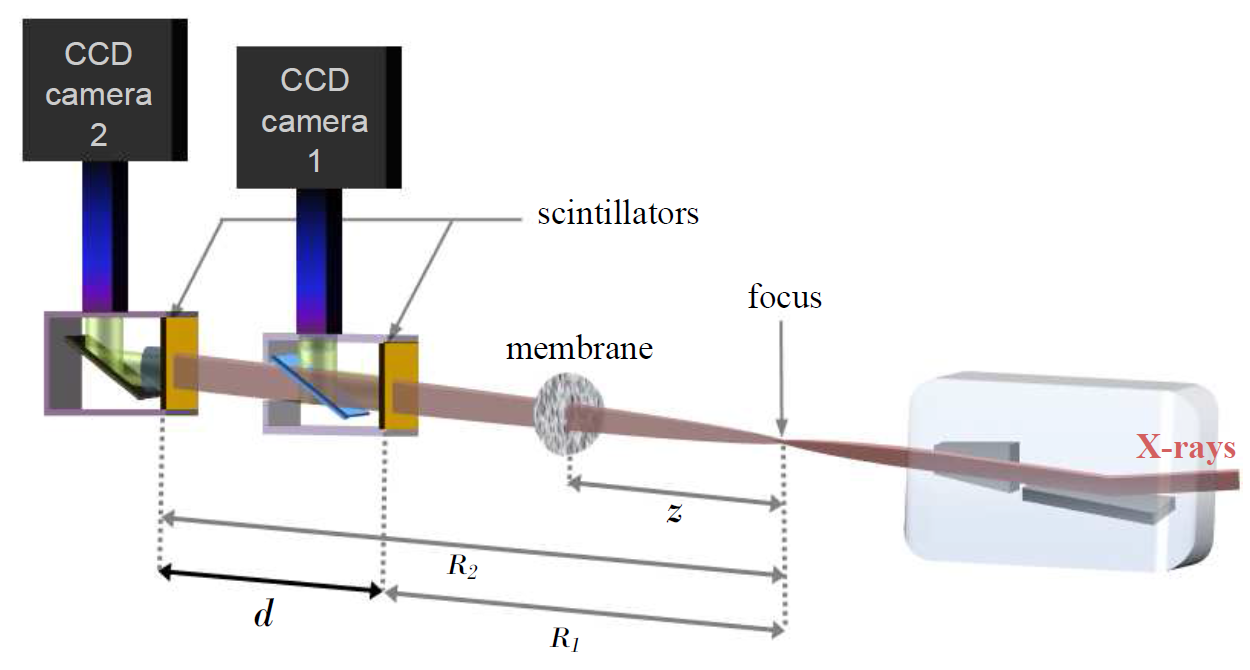
\includegraphics[width=0.9\textwidth]{img/Versuchsaufbau}
		\caption[Versuchsaufbau]{Versuchsaufbau \shortcite{Ber15}{891}}
		\label{fig:versuch}
	\end{center}
\end{figure}

Aus der Verschiebung der Flecken lässt sich die Phase, und somit die Wellenfront des Lichtes rekonstruieren, wozu der Wellenfrontrekonstruktionsalgorithmus verwendet wird. Gemäß \citeauthor{Ber13} besteht dieser aus zwei Teilen, welche im Folgenden genauer beschrieben werden sollen: einer Kalibrierung der \gls{CCD}-Sensoren und der Hauptverarbeitungsroutine der Bilder \shortcite{Ber13}{194}. 

Der Algorithmus soll online (zeitgleich zum Experiment) ausgeführt werden. Die \gls{CCD}-Sensoren haben eine Auflösung von 2048x2048 Pixeln mit einer Farbtiefe von 16 Bit (Graustufen) und liefern bis zu 10 Bilder pro Sekunde.

\subsection{Kalibrierung der CCD-Sensoren}

Während der Kalibrierung findet, gemäß \citeauthor{Ber13}, zuerst eine Parameterinitialisierung statt, in welcher der Kamerafehler der \gls{CCD}-Sensoren in drei Phasen bestimmt wird \shortcite{Ber13}{76 ff., S. 194}. Dazu wird, wie in Abbildung \ref{fig:graph_kalibrierung} gezeigt, zuerst der Median aus einer festen Anzahl dunkler Bilder aufgenommen. Anschließend findet eine Nullfeldkalibrierung bei ungestörter Wellenfront und zum Schluss eine Erkennung von Streueffekten im Detektor statt. Um letzteres zu erreichen werden für jeden \gls{CCD}-Sensor die \gls{N}$^2$ Bilder unter Bewegung der \gls{CCD}-Sensoren aufgenommen, wobei \gls{N} hier gleich der Anzahl der Verschiebungen in X- und Y-Richtung ist. Dadurch lässt sich die horizontale und vertikale Streuung von den einzelnen Sensoren mittels des Speckle-Trackings bestimmen. Da die Kalibrierung lediglich am Anfang des Experiments ein mal durchgeführt werden muss, wird diese im weiteren Verlauf der Arbeit vernachlässigt. 

\begin{figure}[htbp]
	\centering
	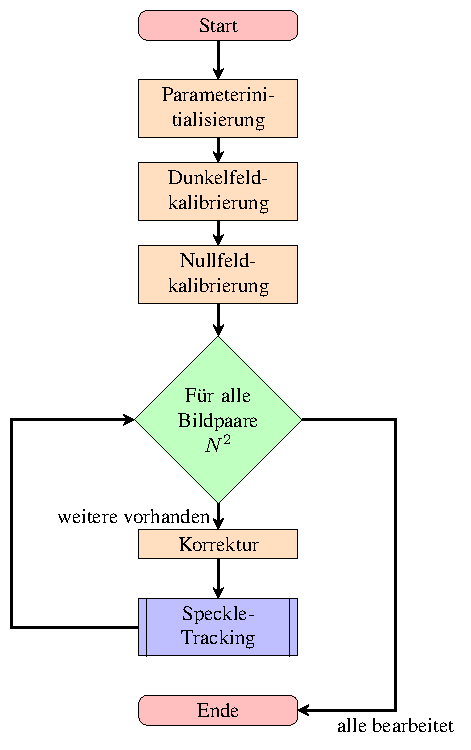
\includegraphics[width=0.45\textwidth]{pdf/graph_init}
	\caption[Kalibrierung]{Programmablaufplan der Kalibrierung (nach \shortcite{Ber13}{85 ff., S. 194} und \cite{Coj17}; angefertigt gemäß DIN 66001 bzw. ISO 5807)}
	\label{fig:graph_kalibrierung}
\end{figure}

\paragraph{Speckle-Tracking}
\label{sec:speckle-tracking}
Ziel des Speckle-Trackings ist es, die Flecken (englisch: speckle) zwischen den \gls{CCD}-Sensoren zu verfolgen, welche von der Fleckenmembran geworfen werden. 
Der von \citeauthor{Ber13} beschriebene Speckle-Tracking-Algorithmus (dargestellt in Abbildung \ref{fig:graph_speckle}) ermittelt zuerst die starre Verschiebung der beiden Sensoren zueinander \shortcite{Ber13}{76 ff., S. 194}. Dies kann mittels festgelegter Werte, Korrelation oder Kreuzkorrelation geschehen. Anschließend werden die Bilder der Sensoren in 35x35 Pixel bzw. 10x10 Pixel große Teilbilder aufgeteilt, damit ein grober Gradient in einem ersten Durchlauf (gezeigt in Abbildung \ref{fig:graph_first}) bestimmt werden kann. Diese Teilbilder liegen hierbei alle in der \gls{ROI}, welche die möglicherweise fehlerbehafteten Bildränder abschneidet. Die Verschiebung der Teilbilder zwischen den beiden Bildern der Sensoren wird mithilfe des von \citeauthor{Lew94} beschriebenen Template-Matching-Prozesses ermittelt \cite{Lew94}. Dieser sucht die Teilbilder des ersten Sensors mit denen des zweiten Sensors, wobei eine Übereinstimmungsmatrix entsteht. Anhand der Positionen der Maxima kann nun die Verschiebung abgelesen werden. Dieser Prozess kann laut \citeauthor{Lew94} durch die Kreuzkorrelation der beiden Teilbilder im Frequenzraum realisiert werden um die Komplexität des Algorithmus zu senken \cite{Lew94}. Damit endet der erste Durchlauf. 
Im weiteren Verlauf werden zuerst stark abweichende Werte herausgefiltert und anschließend werden Ebenen an die horizontalen und vertikalen Verschiebungsmartizen angelegt. Diese sind zur Interpolation nötig, da die Verschiebungsmatrizen lediglich einen Pixel pro Teilbild beinhalten. Sobald die Ebene auf die volle Auflösung des Bildes interpoliert wurde, wird der zweite Durchlauf (gezeigt in Abbildung \ref{fig:graph_second}) durchgeführt. Im diesem Durchlauf werden wieder beide Bilder in Teilbilder unterteilt, diesmal können sich die Teilbilder jedoch überlappen. Die konkrete Anzahl der Teilbilder hängt, gemäß \citeauthor{Coj17}, von drei Variablen ab \cite{Coj17}: der \gls{uap}, der \gls{corrsize} und der \gls{gridResol}. Mittels der Unterabtastperiode lassen sich jeweils \gls{uap} Pixel überspringen, wodurch die effektive \gls{rroi} des Bildes auf \glsdesc{resolution} $\lfloor\glssymbol{resolution}/\gls{uap}^2\rfloor$ reduziert wird. Die \glsfirst{corrsize} \gls{corrsize} gibt die Größe der Teilbilder an. Die \glsfirst{gridResol} bestimmt die Größe des Resultats, indem jeweils ein Teilbild um jeden \gls{gridResol}-ten Punkt im bereits durch Unterabtastung verkleinerten Bild genutzt wird. 
Die Verschiebung der so berechneten Teilbilder wird dann mittels des Template-Matching-Prozesses bestimmt und auf Subpixel-Genauigkeit interpoliert. 
Teilbilder, die im zweiten Durchlauf nicht korrekt zugeordnet werden konnten, werden gesammelt und unter Verwendung von anderen Korrelationsgrößen erneut verarbeitet. Sollten diese Korrelation ebenfalls fehlschlagen, werden die Ergebnisse der fehlerhaften Teilbilder interpoliert. 

\begin{figure}[htbp]
	\centering
	\begin{subfigure}[b]{0.3\textwidth}
		\centering
		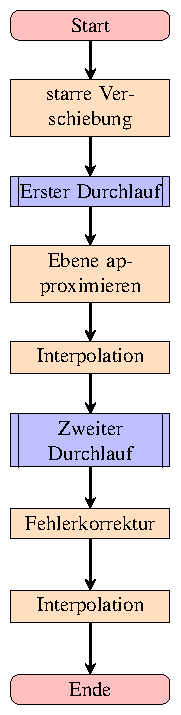
\includegraphics[width=0.5\textwidth]{pdf/graph_speckle}
		\caption[Speckle-Tracking]{Speckle-Tracking-Algorithmus (nach \shortcite{Ber13}{85 ff., S. 194} und \cite{Coj17})}
		\label{fig:graph_speckle}
	\end{subfigure}
	\hfill
	\begin{subfigure}[b]{0.3\textwidth}
		\centering
		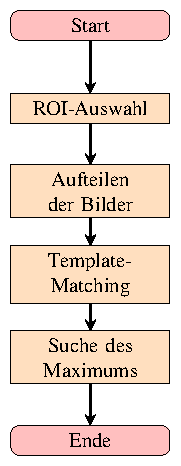
\includegraphics[width=0.6\textwidth]{pdf/graph_first_pass}
		\caption[Erster Durchlauf]{Erster Durchlauf (nach \cite{Ber12} und \cite{Coj17})}
		\label{fig:graph_first}
	\end{subfigure}
	\hfill
	\begin{subfigure}[b]{0.3\textwidth}
		\centering
		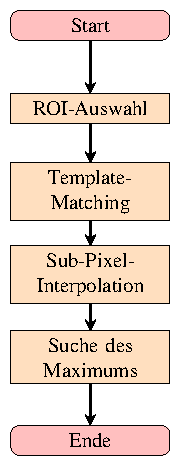
\includegraphics[width=0.6\textwidth]{pdf/graph_second_pass}
		\caption[Zweiter Durchlauf]{Zweiter Durchlauf (nach \shortcite{Ber13}{194}, \cite{Ber12} und \cite{Kov04})}
		\label{fig:graph_second}
	\end{subfigure}
	\caption[Algorithmen]{Programmablaufpläne der Speckle-Tracking-Subroutinen (angefertigt gemäß DIN 66001 bzw. ISO 5807)}
\end{figure}

\subsection{Verarbeitungsroutine der Bilder}

Die von \citeauthor{Ber15} beschriebene Hauptverarbeitungsroutine (siehe Abbildung \ref{fig:graph_hauptroutine}) ähnelt stark der Kalibrierung: Auch hier findet zuerst eine Parameterinitialisierung statt, welche von der Hauptschleife gefolgt wird \shortcite{Ber15}{891}. Diese verarbeitet hier, im Gegensatz zur Kalibrierung, nur jedes Bildpaar. Ein Bildpaar ist exemplarisch in Abbildung \ref{fig:eingabebilder} gezeigt. Innerhalb der Hauptschleife gibt es auch hier die Korrektur der Sensorfehler und das anschließende Speckle-Tracking, dessen Ergebnisse in Abbildung \ref{fig:gradienten} gezeigt sind. Die Korrektur bezieht hierbei die von der Kalibrierung berechneten Ergebnisse, insbesondere die ermittelten Streueffekte der Sensoren. Anders als bei der Kalibrierung, werden hierbei jedoch in der Hauptschleife die beiden Gradientenmatrizen mittels des von \citeauthor{FC88} entwickelten Algorithmus zu einer Phasenmatrix integriert (gezeigt in Abbildung \ref{fig:graph_fc}), was effizient im Frequenzraum möglich ist \cite{FC88}. Die zu in Abbildung \ref{fig:eingabebilder} gezeigten Eingabebildern zugehörige Phasenmatrix ist in Abbildung \ref{fig:ausgabebild} dargestellt. 

\begin{figure}[htbp]
	\centering
	\begin{subfigure}[b]{0.35\textwidth}
		\centering
		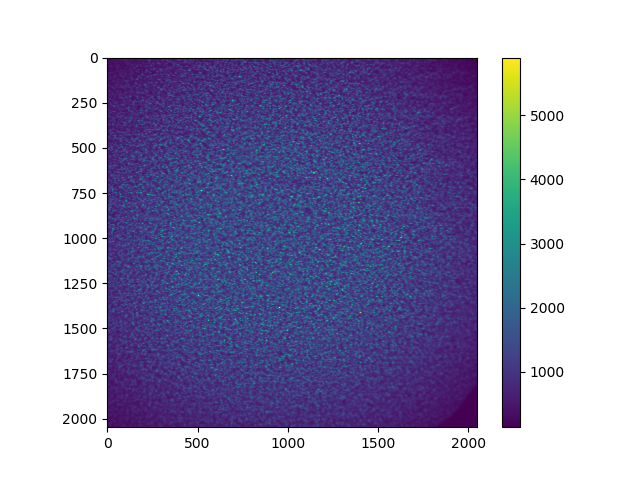
\includegraphics[width=\textwidth]{img/ref_start0001_1-10}
		\caption[Erster Sensor]{Eingabebild des ersten Sensors}
		\label{fig:eingabe_sensor1}
	\end{subfigure}
	\begin{subfigure}[b]{0.35\textwidth}
		\centering
		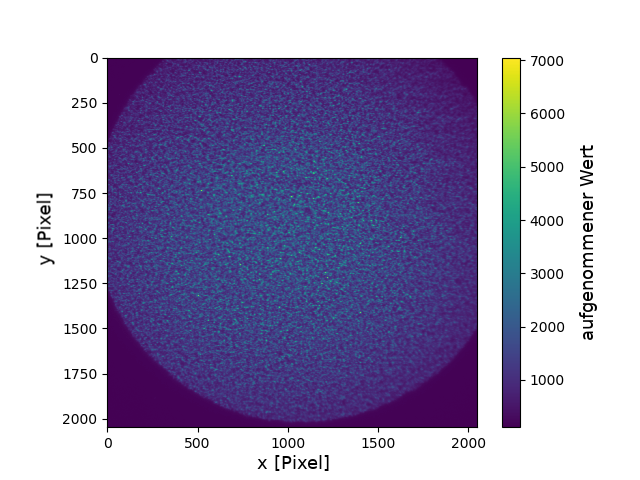
\includegraphics[width=\textwidth]{img/E10001}
		\caption[Zweiter Sensor]{Eingabebild des zweiten Sensors}
		\label{fig:eingabe_sensor2}
	\end{subfigure}
	\caption[Eingabe]{Eingabebilder}
	\label{fig:eingabebilder}
\end{figure}

\begin{figure}[htbp]
	\centering
	\begin{subfigure}[b]{0.35\textwidth}
		\centering
		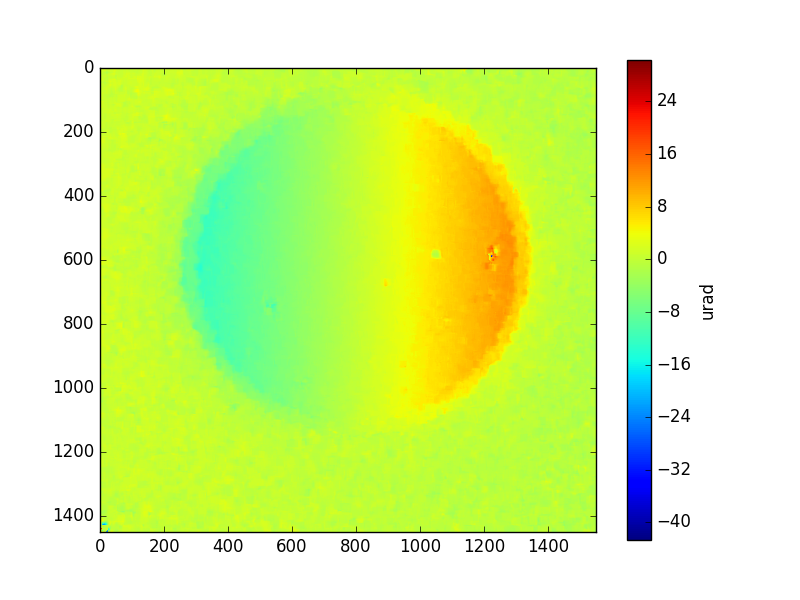
\includegraphics[width=\textwidth]{img/SpeckDisH_E10001_edf_ref_start0001_1-10_edf}
		\caption[Horizontaler Gradient]{Horizontaler Gradient}
		\label{fig:hor_grad}
	\end{subfigure}
	\begin{subfigure}[b]{0.35\textwidth}
		\centering
		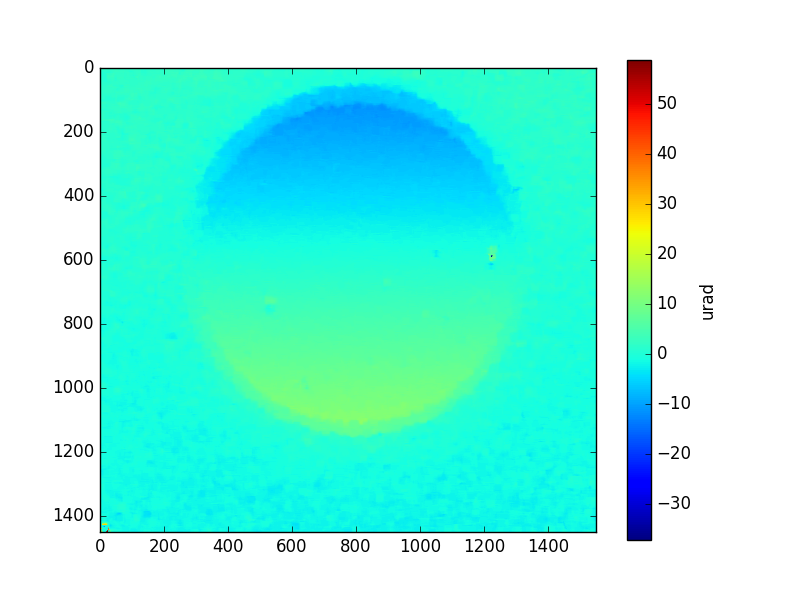
\includegraphics[width=\textwidth]{img/SpeckDisV_E10001_edf_ref_start0001_1-10_edf}
		\caption[Vertikaler Gradient]{Vertikaler Gradient}
		\label{fig:vert_grad}
	\end{subfigure}
	\caption[Gradient]{Gradientenbilder (Ausgabe des Speckle-Tracking)}
	\label{fig:gradienten}
\end{figure}

\begin{figure}[htbp]
	\centering
	\begin{subfigure}[b]{0.35\textwidth}
		\centering
		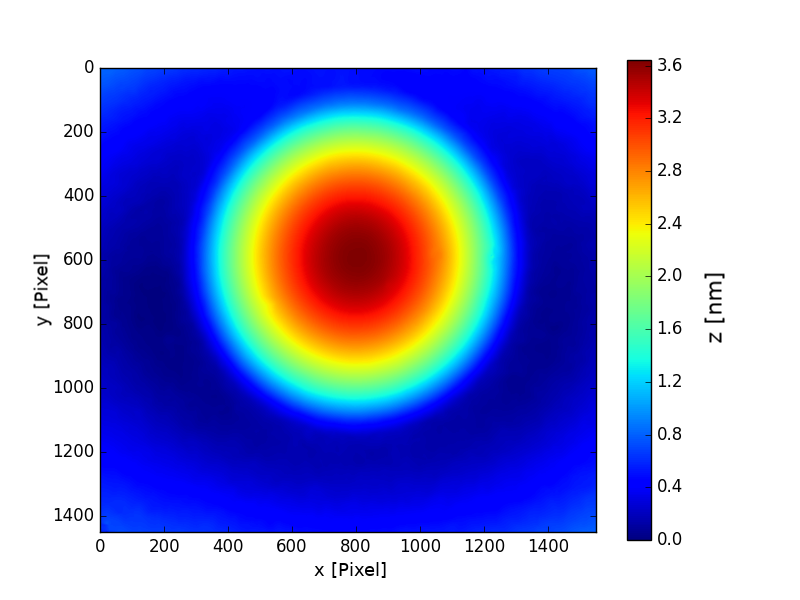
\includegraphics[width=\textwidth]{img/2D_E10001_edf_ref_start0001_1-10_edf}
		\caption[2D Ausgabe]{2D Repräsentation}
		\label{fig:ausgabe_2d}
	\end{subfigure}
	\begin{subfigure}[b]{0.35\textwidth}
		\centering
		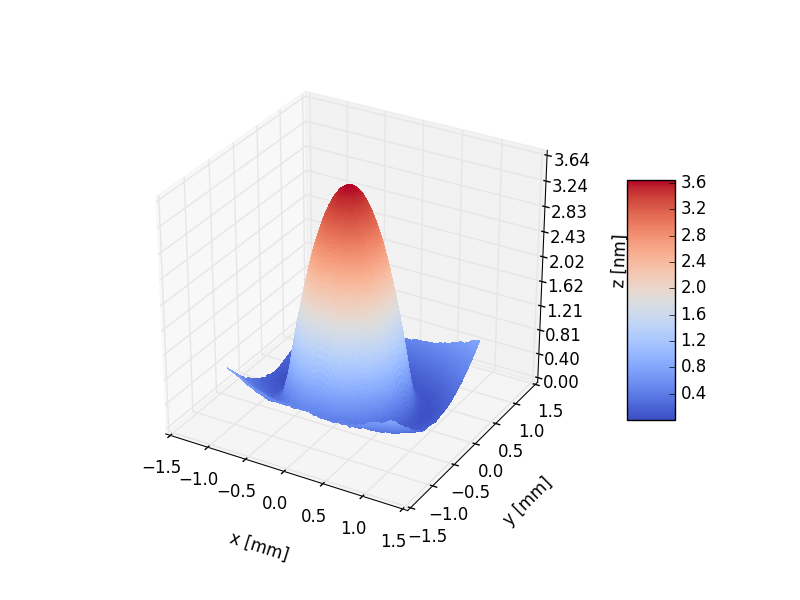
\includegraphics[width=\textwidth]{img/3D_E10001_edf_ref_start0001_1-10_edf}
		\caption[3D Ausgabe]{3D Repräsentation}
		\label{fig:ausgabe_3d}
	\end{subfigure}
	\caption[Ausgabe]{Ausgabe des Algorithmus (Phasenmatrix)}
	\label{fig:ausgabebild}
\end{figure}

\begin{figure}[htbp]
	\begin{subfigure}[b]{0.45\textwidth}
		\centering
		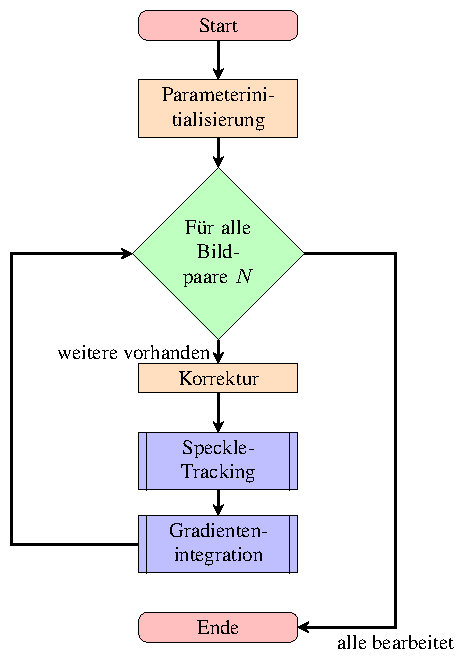
\includegraphics[width=\textwidth]{pdf/graph_main}
		\caption[Hauptroutine]{Hauptroutine (nach \shortcite{Ber13}{194} und \cite{Coj17})}
		\label{fig:graph_hauptroutine}
	\end{subfigure}
	\hfill
	\begin{subfigure}[b]{0.45\textwidth}
		\centering
		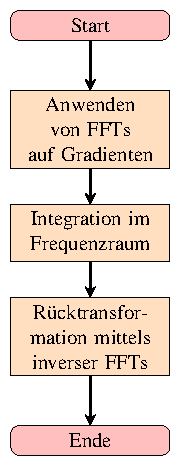
\includegraphics[width=0.4\textwidth]{pdf/graph_fc}
		\caption[Frankot-Chellappa]{Integration der Gradienten gemäß Frankot \textit{et al.} (nach \cite{FC88} und \cite{Kov04})}
		\label{fig:graph_fc}
	\end{subfigure}
	\caption[Algorithmen]{Programmablaufpläne der Hauptroutine (angefertigt gemäß DIN 66001 bzw. ISO 5807)}
\end{figure}

\section{Überblick über den bereits bestehenden Code}

Der bestehende Code wurde von Elena-Ruxandra Cojocaru entwickelt und ist auf GitHub verfügbar \cite{Coj17}. Der Code ist in vier Dateien aufgeteilt. Die Datei \textit{norm\_xcorr.py} nutzt die Schnittstelle zu der in OpenCV implementierten Template-Matching-Funktion \cite{SA17}. Alle Helferfunktionen, insbesondere die des Speckle-Trackings und die der Integration der Gradienten, befinden sich in der \textit{func.py}. Der Code der Kalibrierung befindet sich in der \textit{detectorDistortion.py} Datei und der der Hauptroutine befindet sich in der Datei \textit{wavefront.py}. 

\subsection{norm\_xcorr.py}

Die Datei \textit{norm\_xcorr.py} enthält alle Funktionen, die für das Template-Matching benötigt werden. Darunter ist die Funktion \textit{norm\_xcorr()}, welche lediglich als Schnittstelle für die Template-Matching Funktion aus OpenCV dient. Sie nimmt als Argumente ein Template, ein Suchfeld und optional den Namen des gewünschten Algorithmus entgegen und gibt die Übereinstimmungsmarix, die Position und den Wert des Maximums und des Minimums zurück.

Die zweite Funktion in dieser Datei ist die \textit{nxcorr\_disp()}-Funktion, welche die Übereinstimmungsmatrix an relevanten Stellen, wo die Übereinstimmung am höchsten ist, auf ein Subpixel-Level verfeinert. Dazu nimmt diese Funktion das Ergebnis der \textit{norm\_xcorr()}-Funktion entgegen und gibt die Position sowie den Wert des neuen Maximums und das Signal-Rausch-Verhältnis zurück. 

\subsection{func.py}

Die \textit{func.py} enthält die meisten Helferfunktionen. Dazu gehören unter anderem Funktionen zur \gls{ROI}"=Auswahl und verschiedene Filterfunktionen. 

Des Weiteren befinden sich in dieser Datei auch die Funktionen \textit{computerCorrField()} und \textit{correction()}. \textit{computerCorrField()} berechnet aus Bildern an einem vorgegebenen Pfad entweder das mediangefilterte Bild für die Dunkelfeld-Kalibrierung oder das durchschnittsgefilterte Bild für Nullfeld-Kalibrierung. Mithilfe der \textit{correction()} Funktion können nun diese berechneten Korrekturbilder auf Eingabebilder mittels Subtraktion für die Dunkelfeld-Kalibrierung oder mittels Division für die Nullfeld-Kalibrierung angewendet werden.

Zwei weitere wichtige Funktionen sind \textit{firstPass()} und \textit{cpCorr()}, welche den ersten (\textit{firstPass()}) und zweiten Durchlauf (\textit{cpCorr()}) implementieren. Diese sind damit Teil des Speckle-Trackings-Algorithmus, welcher in der \textit{crossSpot4()}-Funktion implementiert ist.

Die letzte wichtige Funktion im \textit{func.py}-Skript ist die \textit{frankot\_chellappa()}-Funktion, welche aus Gradientenfeldern eine dreidimensionale Rekonstruktion berechnet. Dies wird nach dem Speckle-Tracking verwendet. Um dies effizient und schnell zu erreichen, werden die Eingabematrizen mittels \glspl{FFT} in den Frequenzraum transformiert, dort nach Formel 21 des von \citeauthor{FC88} beschriebenen Algorithmus addiert und wieder zurück transformiert \shortcite{FC88}{443}. 

\subsection{wavefront.py}

Das letzte Skript, \textit{wavefront.py}, beinhaltet den eigentlichen Rekonstruktionsalgorithmus, welcher sich besonders in der Initialisierungsphase sehr stark dem \textit{detectorDistortion.py}-Skript ähnelt, welches die Kalibrierung der\gls{CCD}-Sensoren implementiert. Die Hauptroutine wird jetzt, wie in Abbildung \ref{fig:graph_hauptroutine} veranschaulicht, nur einmal für jedes Bildpaar statt für jede Kombination aus Eingabebildern ausgeführt. Innerhalb dieser Routine wird das entsprechende Bildpaar samt Stellung Positionierungsmotoren der \gls{CCD}-Sensoren geladen und mittels der \textit{correction()}-Funktion korrigiert. Da die Pixelgröße zwischen den Sensoren unterschiedlich sein kann, wird hierfür eine Interpolation durchgeführt, die dieses Problem beheben soll. Bevor das Speckle-Tracking mittels der \textit{crossSpot4()}-Funktion ausgeführt wird, können optional noch ein Gauß-Filter, ein Mittelwertfilter und ein Erosionsfilter angewendet werden. Danach werden die Zwischenergebnisse gespeichert und die endgültige Wellenfront wird mittels der \textit{frankot\_chellappa()}-Funktion rekonstruiert und gespeichert. 

\section{Die wichtigsten Funktionen}

\subsection{norm\_xcorr()}

Die \textit{norm\_xcorr()}-Funktion ist die direkte Schnittstelle für die in OpenCV implementierte \textit{matchTemplate()}-Funktion. Hierbei wird eine Matrix aus Übereinstimmungen mittels Faltung erstellt, die an jedem Pixel mit einem Wert zwischen $-1$ und $1$ angibt, wie ähnlich sich die Bilder sind. Diese Funktion ist Teil des Speckle-Tracking-Algorithmus, der dafür zuständig ist, die Verschiebung der Wellenfront zwischen den beiden \gls{CCD}-Sensoren zu ermitteln. Standardmäßig wird hierbei der Kreuzkorrelationskoeffizient verwendet. 

\subsection{nxcorr\_disp()}

Aufgabe dieser Funktion ist es, den Punkt der maximalen Übereinstimmung auf ein Subpixel-Level zu verfeinern. Dazu wird der Gradient der Pixelwerte in der Nachbarschaft des Maximums gebildet und anschließend interpoliert. Im Gesamtalgorithmus wird dieser Schritt direkt nach dem Template-Matching als Teil des Speckle-Trackings ausgeführt.

\subsection{frankot\_chelappa()}

Die \textit{frankot\_chellappa()}-Funktion nutzt den von \citeauthor{FC88} vorgeschlagenen Algorithmus um aus vorgegebenen Gradientenfeldern ein dreidimensionales Bild zu rekonstruieren \cite{FC88}. Der hier bereits vorliegende Code basiert auf dem Matlab-Code von \citeauthor{Kov04} \cite{Kov04}. Die \textit{frankot\_chellappa()}-Funktion wird nach dem Speckle-Tracking aufgerufen und nutzt die durch das Tracking ermittelten Gradientenmatrizen um die Wellenfront dreidimensional zu rekonstruieren. 